\documentclass{article}
\usepackage[utf8]{inputenc}
\usepackage{authblk} % To make the adress/email look ok
\usepackage{amsmath} % To use mathematics
\usepackage{tcolorbox} % To use box around text

\title{Labreport project}

\author{Sara Alterkawi}

\affil{Dataingenjör, Group 1}

\date{Oct 2021}

\begin{document}

\maketitle

\section{Introduction}
In game 2048. You merge similar tiles by moving them in any of the four directions to make "bigger" tiles. After each move, a new tile appears at random empty position with a value of either 2 or 4. The game terminates when all the boxes are filled and there are no moves that can merge tiles, or you create a tile with a value of 2048.
This lab is about developing AI that outperforms to solve a game 2048.

% Explain del1
\section{Del 1}
In This task I will use the agents (AI) that I developed in Lab 3. And I will describe in detail all the lines that I AI executes (in project).

\subsection{Code}
The code used:

\begin{tcolorbox}
\begin{verbatim}
function direction = project(A)
B = convertToLogBoard(A);
d = {'up', 'down', 'right', 'left'};
heuristicValues = zeros(1,4);
for i = 1:length(d)
    Bnew = slide(B,d{i});
    if isequal(Bnew ,B);
        heuristicValues(i) = -Inf;
    else
        heuristicValues(i) = ... 
            heuristic0(Bnew);
    end
end
[valueMax, iMax] = max(heuristicValues);
direction = d{iMax};
end
function u = heuristic0(B)
u = sum(B(:) == 0);
end
function u = heuristic1(B)
u  =  - sum(B(:)); 
end
function u = heuristic2(B)
alpha = 0.25; 
u =(1-alpha)*heuristic0(B) + alpha*heuristic1(B);
end
function u = heuristic4(B)
u = heuristic0(B)+heuristic1(B)+heuristic2(B);
end
function B =convertToLogBoard(B)
B(isnan(B)) = 1;
B = log2(B);
end
\end{verbatim}
\end{tcolorbox}

\subsection{Code explanation}
The code explanation:

\begin{tcolorbox}
\begin{verbatim}
function direction = project(A)
\end{verbatim}
\end{tcolorbox}
Define function of direction and at each step the game ask of the input of direction from this function and the A here is the board.

\begin{tcolorbox}
\begin{verbatim}
B = convertToLogBoard(A);
\end{verbatim}
\end{tcolorbox}
Here it convert A to another representation

\begin{tcolorbox}
\begin{verbatim}
d = {'up', 'down', 'right', 'left'};
\end{verbatim}
\end{tcolorbox}
The set of actions in the game to select from

\begin{tcolorbox}
\begin{verbatim}
heuristicValues = zeros(1,4);
\end{verbatim}
\end{tcolorbox}
Making a vector of four values computing the heuristic values of four direction in for loop repeating some action over and

\begin{tcolorbox}
\begin{verbatim}
for i = 1:length(d)
\end{verbatim}
\end{tcolorbox}
i is the counter of for loop which is here four

\begin{tcolorbox}
\begin{verbatim}
Bnew = slide(B,d{i});
\end{verbatim}
\end{tcolorbox}
Predictive state from action i which is from slide code and d direction

\begin{tcolorbox}
\begin{verbatim}
if isequal(Bnew ,B);
\end{verbatim}
\end{tcolorbox}
if action i does not change the state    

\begin{tcolorbox}
\begin{verbatim}
heuristicValues(i) = -Inf;
\end{verbatim}
\end{tcolorbox}
Put heuristic to be -infinity

\begin{tcolorbox}
\begin{verbatim}
else
\end{verbatim}
\end{tcolorbox}
Otherwise, evaluate the state.

\begin{tcolorbox}
\begin{verbatim}
heuristicValues(i) = ...
\end{verbatim}
\end{tcolorbox}
To take the i value from

\begin{tcolorbox}
\begin{verbatim}
heuristic0(Bnew);
\end{verbatim}
\end{tcolorbox}
To give Bnew a heuristic0

\begin{tcolorbox}
\begin{verbatim}
end
end
\end{verbatim}
\end{tcolorbox}

\begin{tcolorbox}
\begin{verbatim}
[valueMax, iMax] = max(heuristicValues);
\end{verbatim}
\end{tcolorbox}
Find the action of the maximum heuristic value

\begin{tcolorbox}
\begin{verbatim}
direction = d{iMax};
\end{verbatim}
\end{tcolorbox}
Output the string

\begin{tcolorbox}
\begin{verbatim}
end
\end{verbatim}
\end{tcolorbox}

\begin{tcolorbox}
\begin{verbatim}
function u = heuristic0(B)
u = sum(B(:) == 0);
end
\end{verbatim}
\end{tcolorbox}
The number of bricks that are zero

\begin{tcolorbox}
\begin{verbatim}
function u = heuristic1(B)
u  =  - sum(B(:)); 
end
\end{verbatim}
\end{tcolorbox}
the negative sum of the values of the bricks (remember they are in logarithm, so its not the original values being summed)

\begin{tcolorbox}
\begin{verbatim}
function u = heuristic2(B)
alpha = 0.25;
u =(1-alpha)*heuristic0(B) + alpha*heuristic1(B);
end
\end{verbatim}
\end{tcolorbox}
In the new function we define a new heuristics which is a mix of heuristic 0 and heuristic 1

\begin{tcolorbox}
\begin{verbatim}
function u = heuristic4(B)
u = heuristic0(B)+heuristic1(B)+heuristic2(B);
end
\end{verbatim}
\end{tcolorbox}
In the new function we define a new heuristics which is a mix of heuristic0, heuristic1 and heuristic2

\begin{tcolorbox}
\begin{verbatim}
function B =convertToLogBoard(B)
B(isnan(B)) = 1;
\end{verbatim}
\end{tcolorbox}
It checks nan and convert it to one

\begin{tcolorbox}
\begin{verbatim}
B = log2(B);
\end{verbatim}
\end{tcolorbox}
Compute the exponent using the log

\begin{tcolorbox}
\begin{verbatim}
end
\end{verbatim}
\end{tcolorbox}

\subsection{The board after running the game}

% To Upload AIBoard figure to the project
\begin{figure}[h!]
\centering
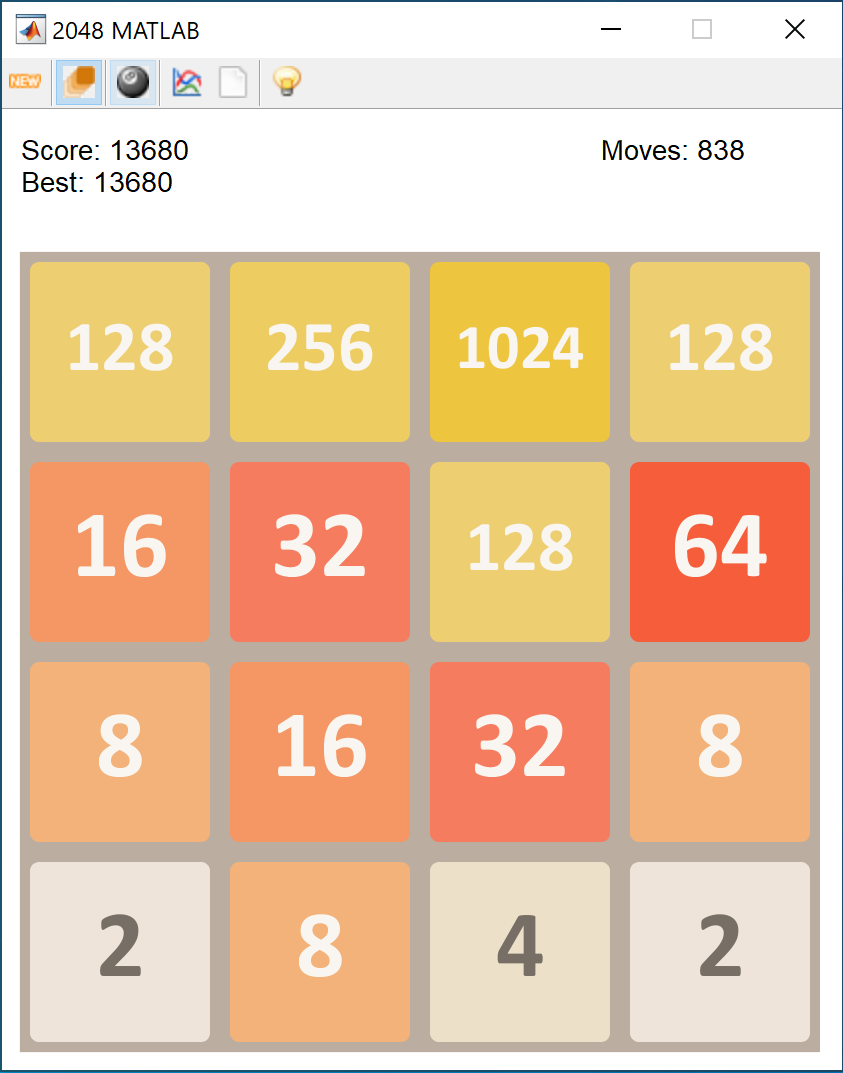
\includegraphics[width=7cm]{proj.png}
\label{fig:MyAI4 results}
\end{figure}

\subsection{Comparison between AI4 and my own AI}
\begin{tcolorbox}
\begin{verbatim}
g4 = Game2048Simulator(@myAI4);
simulate(g4, 300)
viewResult(g4, 15)

pro = Game2048Simulator(@project);
simulate(pro, 300)
viewResult(pro, 15)

scores_4=g4.Result.Score;
scores_p=pro.Result.Score;
[h,p]= ttest2(scores_4,scores_p,'Tail','left');
\end{verbatim}
\end{tcolorbox}

% To Upload my project histogram figure to the project
\begin{figure}[h!]
\centering
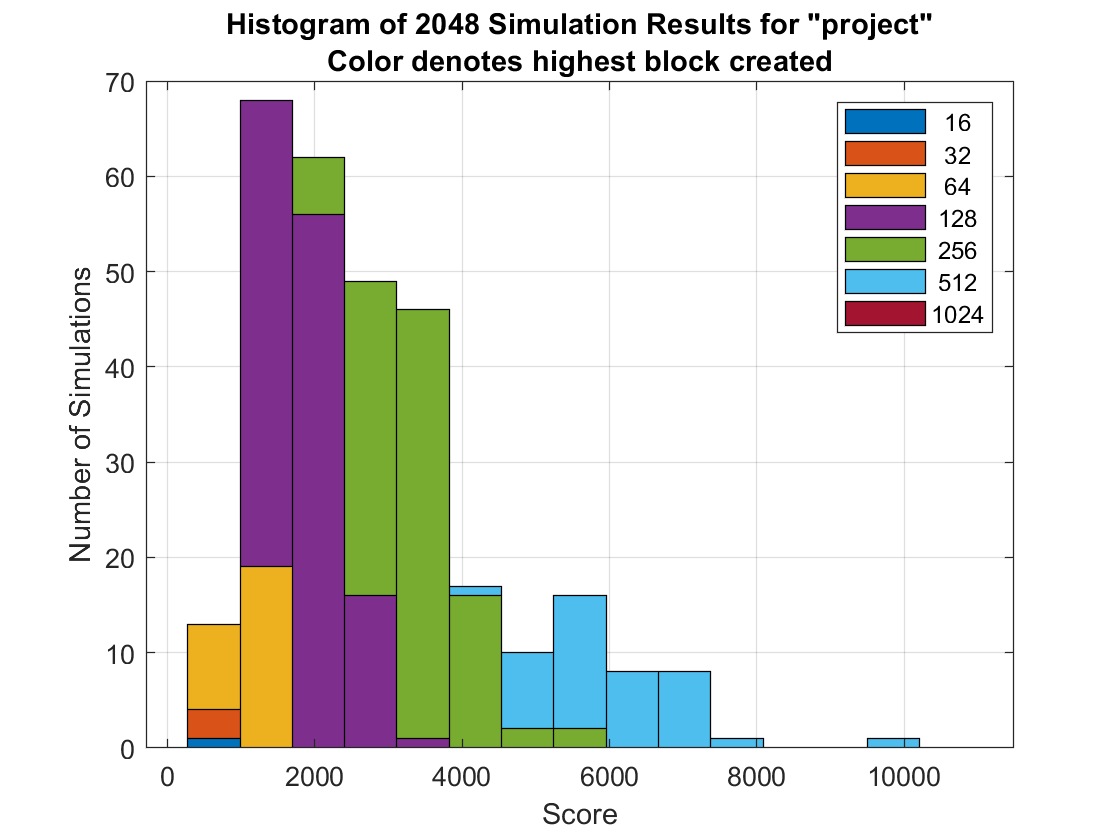
\includegraphics[width=7cm]{project_score.png}
\label{fig:MyAI4 results}
\end{figure}

% To Upload myAI4 histogram figure to the project
\begin{figure}[h!]
\centering
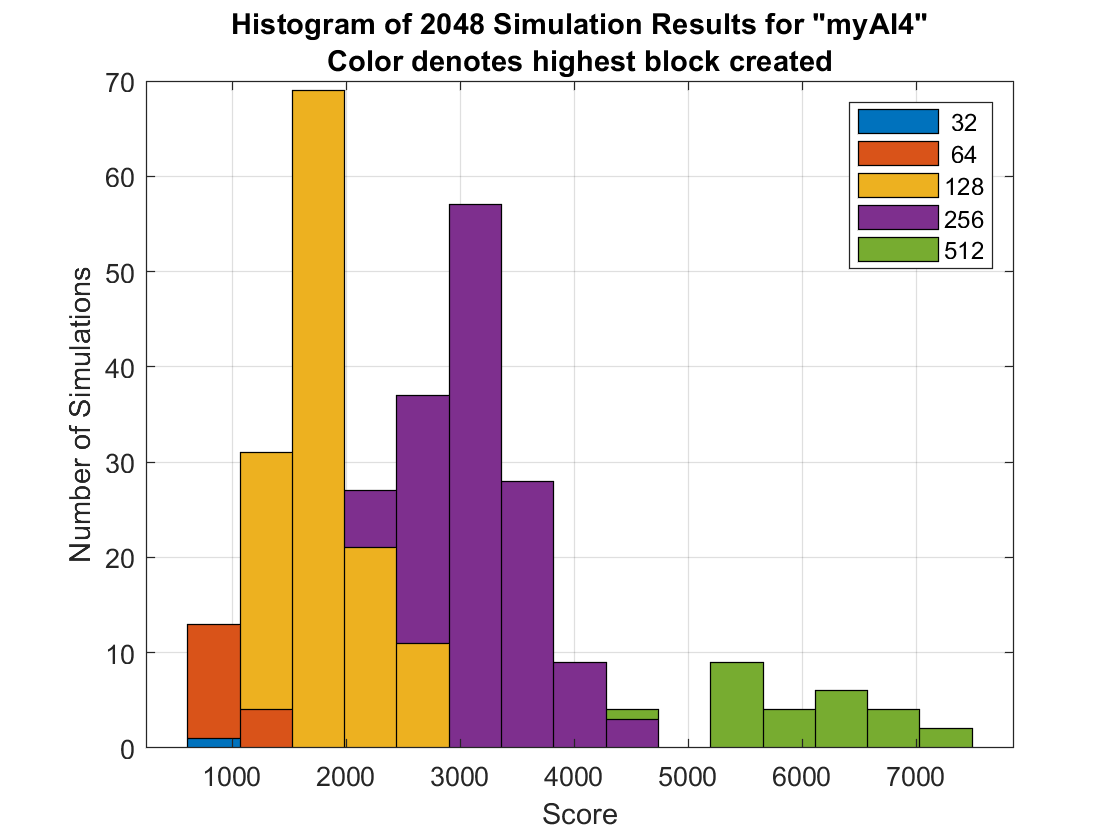
\includegraphics[width=7cm]{myAI4_score.png}
\label{fig:MyAI4 results}
\end{figure}

\subsection{Comparison results}
The command window shows us the result which shown in the figure

% To Upload ttest figure to the project
\begin{figure}[h!]
\centering
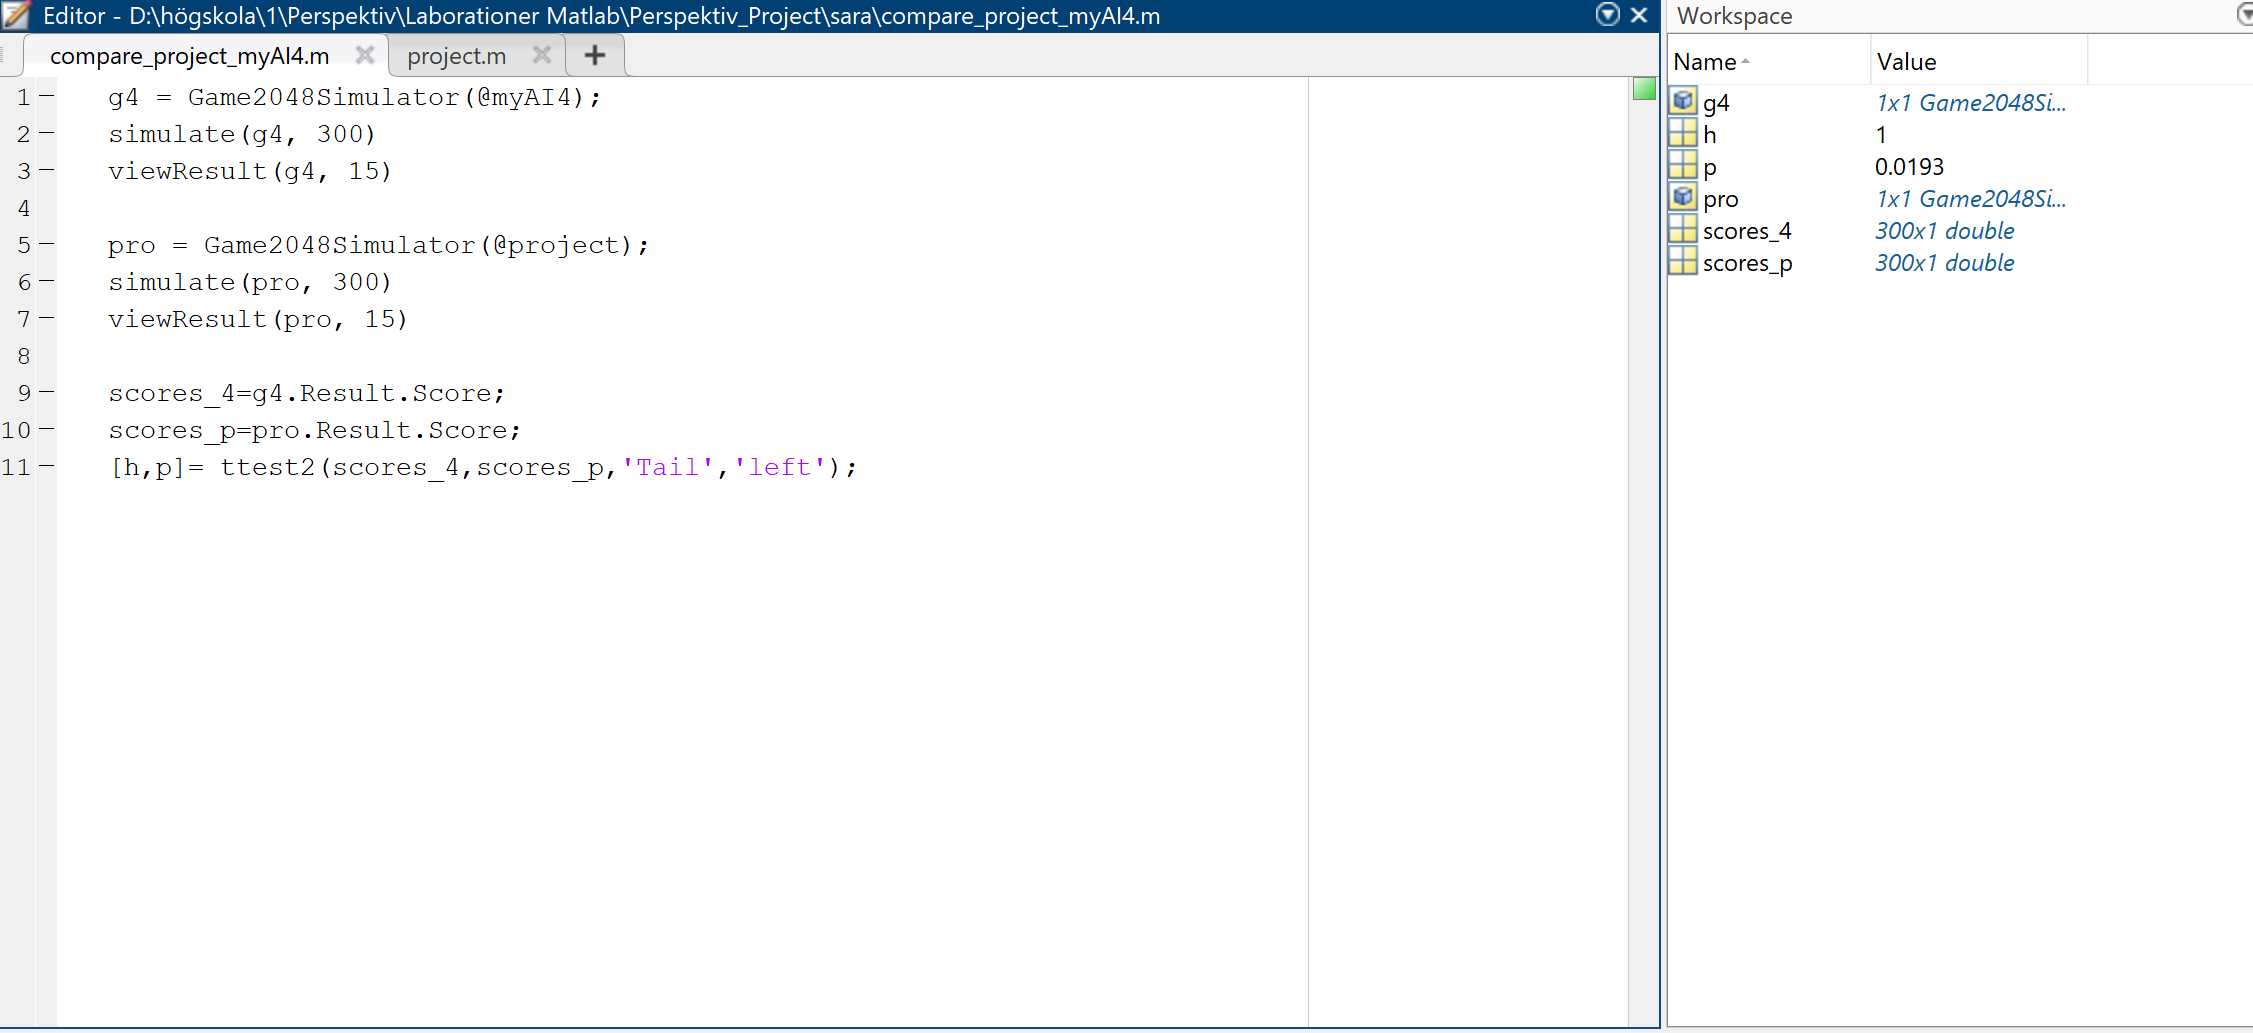
\includegraphics[width=7cm]{ttest2.png}
\label{fig:MyAI4 results}
\end{figure}

\subsection{Conclusion of Comparison results}
P-value is the significance value of the test. which accept the one hypothesis and p value is bigger than 5\%. using the tail left we got the result scores\_p $>$ scores\_4 which mean that the combination of three heuristics is better than one heuristic

\end{document}